\begin{figure}[tb]
\centering
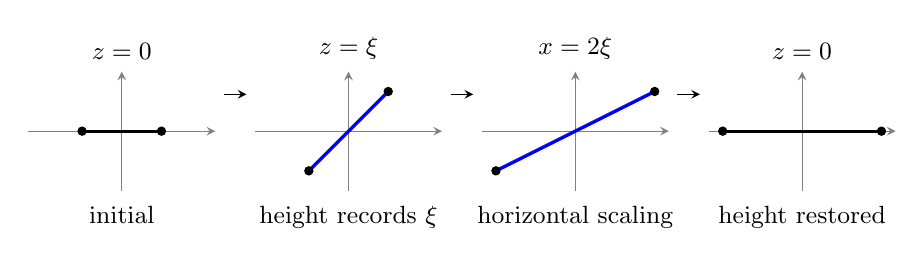
\begin{tikzpicture}[x=0.72cm,y=0.72cm,>=stealth]
\foreach \dx/\lab in {0/{initial},4/{height records $\xi$},8/{horizontal scaling},12/{height restored}}{
 \begin{scope}[shift={(\dx,0)}]
 \draw[->,gray] (-1.65,0)--(1.65,0);
 \draw[->,gray] (0,-1.05)--(0,1.05);
 \node[below,align=center,font=\small] at (0,-1.15) {\lab};
 \end{scope}}
\draw[very thick] (-0.7,0)--(0.7,0);
\draw[very thick,blue] (3.3,-0.7)--(4.7,0.7);
\draw[very thick,blue] (6.6,-0.7)--(9.4,0.7);
\draw[very thick] (10.6,0)--(13.4,0);
\foreach \x/\y in {-0.7/0,0.7/0,3.3/-0.7,4.7/0.7,6.6/-0.7,9.4/0.7,10.6/0,13.4/0}
 \fill (\x,\y) circle (1.7pt);
\draw[->] (1.8,0.65)--(2.2,0.65);
\draw[->] (5.8,0.65)--(6.2,0.65);
\draw[->] (9.8,0.65)--(10.2,0.65);
\node[above,font=\small] at (0,1.1) {$z=0$};
\node[above,font=\small] at (4,1.1) {$z=\xi$};
\node[above,font=\small] at (8,1.1) {$x=2\xi$};
\node[above,font=\small] at (12,1.1) {$z=0$};
\end{tikzpicture}
\caption{A slice of the sheet-scaling triple, in local coordinates with
vertical coefficient one and horizontal factor $\lambda=2$.  A vertical shear records the initial horizontal
offset in height; the horizontal shear doubles that offset; the last
vertical shear returns the sheet to height zero.  Nearby normal offsets
are contracted by $1/2$, as the determinant-one formula in the text shows.
Each depicted segment is the image of the entire initial segment.}
\label{sv:normal-figure}
\end{figure}
